\chapter{Conception et implémentation}
\label{chapterImpl}

Ce chapitre traitera de ce qui a été conçu, et implémenté durant le stage.
\section{Technologies utilisées}
Les technologies étaient fixées d'avance par les contraintes du projet.

\begin{itemize}
	\item Le langage de programmation est le \brand{C++}.
	\item Les cadriciels utilisés sont \brand{Qt} pour l'interface et \brand{Jamoma} pour la bibliothèque de base.
	\item La majorité du développement se fait sous \brand{Mac OS X}.
	\item Les outils de gestion de projet sont \brand{Dropbox}, \brand{GitHub} et \brand{Asana}.
\end{itemize}

Néanmoins, j'ai décidé très tôt d'entreprendre un portage des librairies nécessaires sous systèmes \brand{Linux}, de manière à pouvoir faire fonctionner le logiciel sur systèmes embarqués.

\section{Organisation du travail}
\subsection{Choix effectués}
\subsubsection{Prototypage}
Pour prototyper rapidement des applications utilisant les réseaux de Petri, j'ai choisi d'utiliser \brand{PetriNet API}, en raison de la simplicité d'utilisation de cette bibliothèque. En la prenant en main, j'ai rapidement compris le fonctionnement des réseaux de Petri.
J'ai aussi utilisé \brand{Qt} pour les interfaces graphiques, en raison de ma connaissance préalable du sujet.

\subsubsection{Technologie réseau}
Pour le réseau, j'ai très vite choisi d'utiliser \gls{zeroconf}. En effet, la majorité des utilisateurs étant des artistes, ils ne devraient pas avoir à se poser la question des adresses IP et ports à utiliser.
Néanmoins, j'ai gardé la possibilité de connexions entre machines en utilisant un couple \verb|IP:port|, principalement pour permettre un fonctionnement sur Internet.
Pour la communication inter-machines, j'ai choisi d'utiliser \brand{OSC}. En effet, c'est le protocole utilisé dans \brand{i-score} et \brand{Jamoma}, et des bibliothèques pour s'en servir étaient déjà présentes.

\subsection{Fonctionnement en équipe}
Étant dans un travail en équipe et open-source, j'ai été confronté de multiples fois à des problèmes courants dans cette situation : 

\begin{itemize}
	\item Dans le cas d'implémentations divergentes. Une partie de mon travail étant situé sur les branches de développement, et n'étant pas le seul à avoir les droits de commit, il arrivait parfois que les builds soient cassés.
	\item Dans le cas de contributions à mon travail. Il est arrivé que des contributeurs extérieurs fassent des requêtes (\textit{pull requests}) sur mon code, afin d'ajouter des fonctionnalités.
\end{itemize}

Les dépôts étant publics, il m'est aussi arrivé d'avoir des questions sur le fonctionnement de mon code d'utilisateurs extérieurs.

\section{Réalisations}
\subsection{Logiciel de test de répartition}
Ma première impulsion a été de créer un logiciel, nommé \brand{dpetri} (pour \textit{distributed petri}) permettant d'exécuter un réseau de Petri sur un réseau informatique, en associant à chaque machine du réseau des transitions (la valeur des places est partagée intelligemment entre les deux nœuds qui y sont attenants).

Les échanges de messages se font par \ac{OSC}, et il n'y a pas de gestion du retard intégrée. Cette tâche reste à appliquer à la main, ou avec un algorithme externe, sur les réseaux de Petri passés en entrée.

La librairie sous-jacente utilisée était à la base \brand{PetriNet API}~\cite{lohmann2009petri}. Néanmoins, en voulant tester sur \brand{Android}, la librairie n'a pu fonctionner car elle requiert un fichier binaire propriétaire, qui n'est compilé que pour architectures \brand{x86}. J'ai donc réimplémenté une structure de réseau de Petri qui suit l'architecture de \brand{PetriNet API}, mais en offrant uniquement les capacités nécessaires au logiciel. Ceci dit, la visualisation en temps-réel n'est alors plus possible.

Le logiciel affiche le retard à l'exécution d'une transition. L'interface, visible en \cref{fig.dpetri}, est écrite en \brand{Qt}, et utilise \brand{ZeroConf} avec une architecture client / serveur.
\begin{figure}[H]
	\centering
	\begin{tabu} to \linewidth {cc}
	\begin{subfigure}{.5\textwidth}
		\centering
		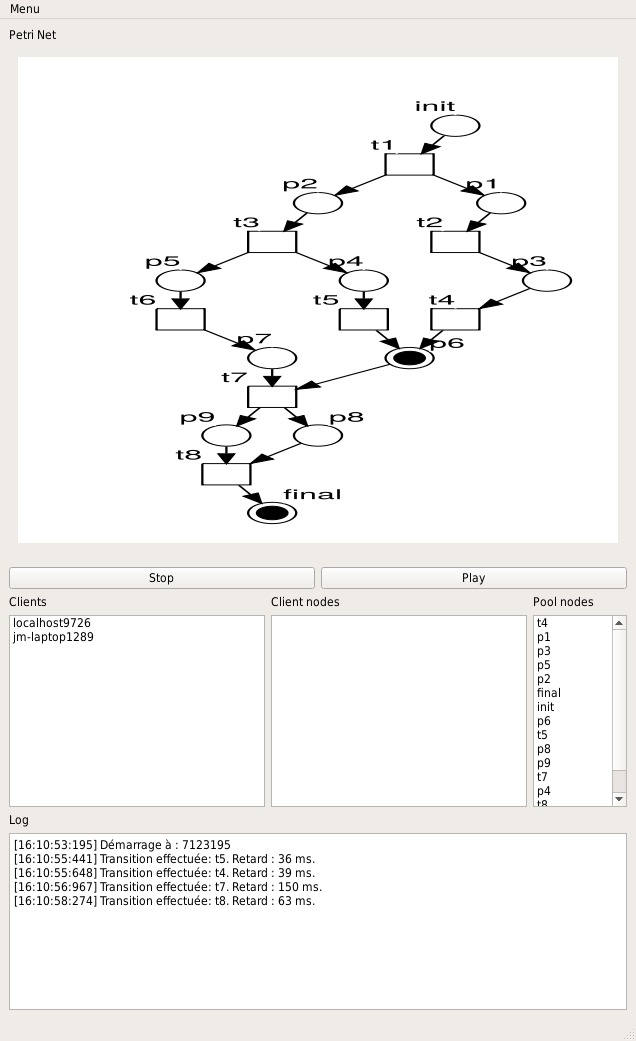
\includegraphics[scale=0.3]{images/dpetriServer.png}
		\caption{Vue serveur}
	\end{subfigure} &
	\begin{subfigure}{.5\textwidth}
		\centering
		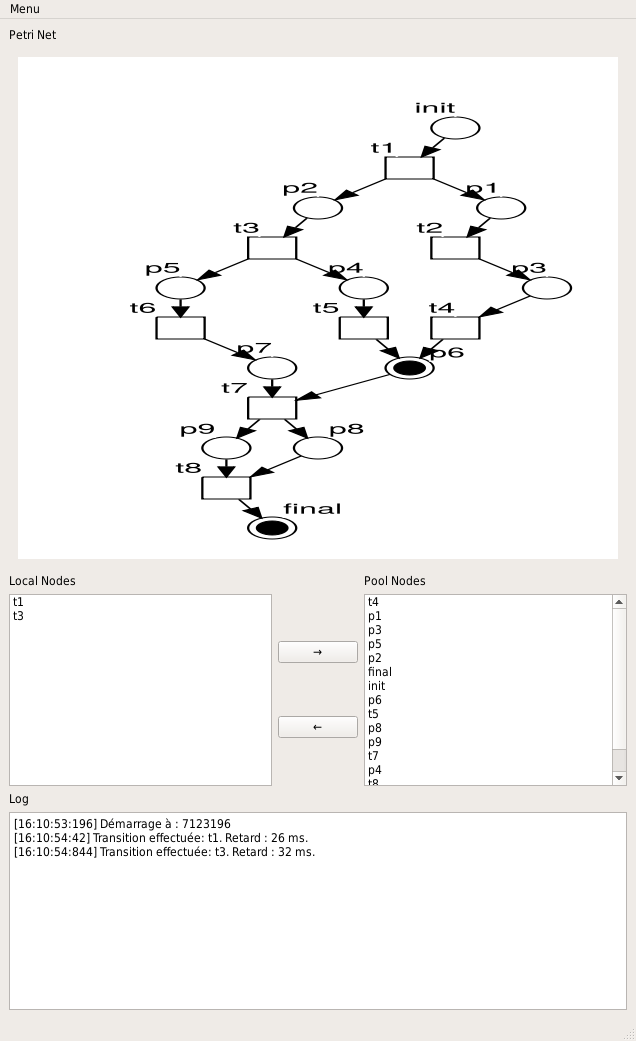
\includegraphics[scale=0.3]{images/dpetriClient.png}
		\caption{Vue client}
	\end{subfigure}
	\end{tabu}
	
	\begin{subfigure}{.5\textwidth}
		\centering
		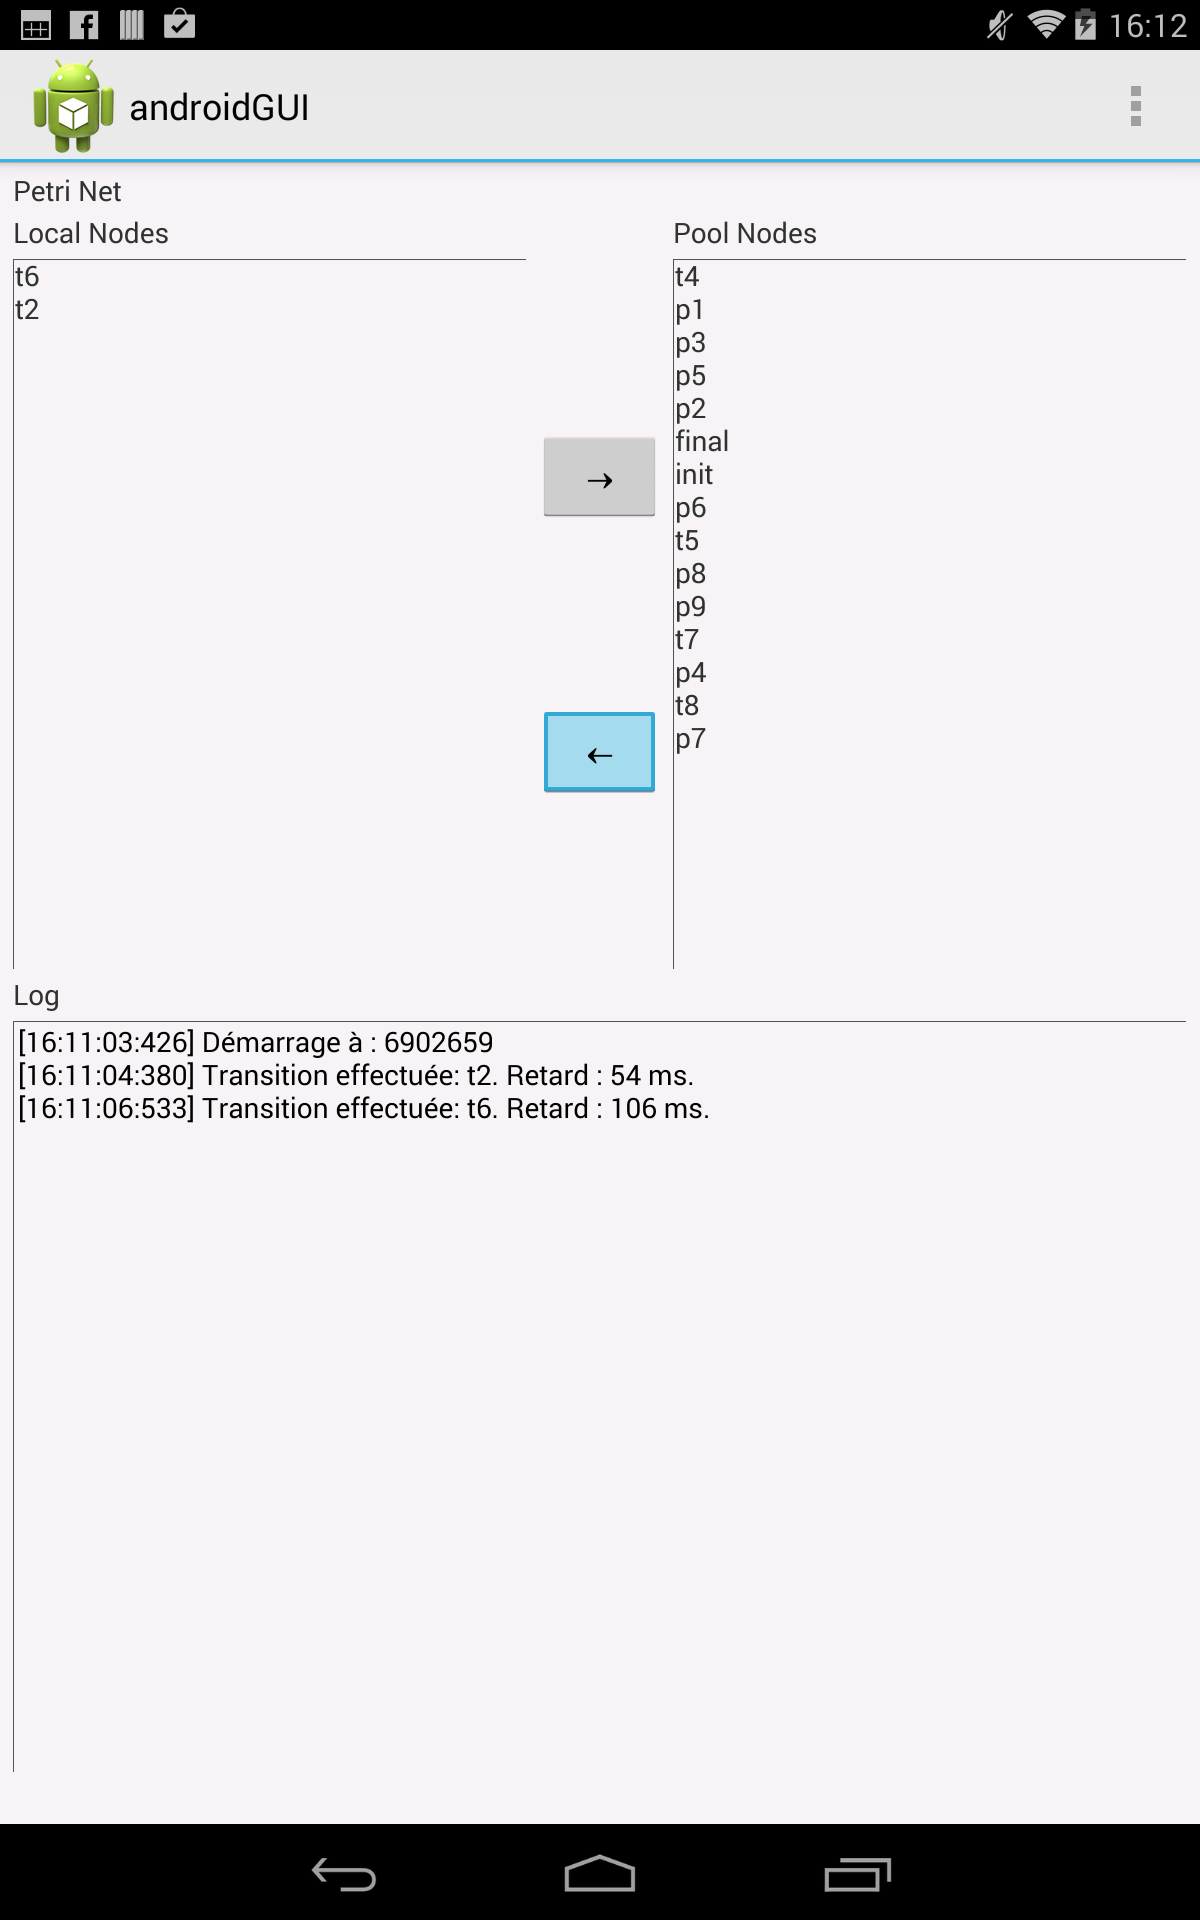
\includegraphics[scale=0.16]{images/dpetriAndroid.png}
		\caption{Vue client Android}
	\end{subfigure}
	
	\caption{Présentation des différentes vues du logiciel de test, \brand{dpetri}}
	\label{fig.dpetri}
\end{figure}

Le code source est présent sur \brand{GitHub} à l'adresse \url{https://github.com/jcelerier/dpetri}.

\subsection{Portage sous GNU/Linux et Android}
Afin d'avoir une exécution des scénarios interactifs sur embarqué, il était nécessaire de porter \brand{Jamoma} et \brand{i-score} sous systèmes Linux (\brand{Android} étant très semblable).

Cela a nécessité un portage du processus de construction logicielle (\textit{build system})  de \brand{Jamoma}, un script Ruby personnalisé, vers \gls{CMake}.

Réaliser ce développement a également permis de distribuer \brand{i-score} sous \gls{macports}, et a ouvert de nouvelles perspectives de développement pour l'embarqué sur le logiciel; de plus, un système d'\gls{contintegr} est désormais envisageable.

Un portage a aussi été réalisé sous \brand{BeagleBoard}, pour offrir un \textit{proof-of-concept} de fonctionnement sur périphérique embarqué courant. Cependant, le moteur d'exécution d'\brand{i-score}, travaillant à une fréquence de $\num{1} \si{\kHz}$, l'exécution demandait trop de ressources pour avoir un fonctionnement correct.

J'ai travaillé sur les branches \texttt{feature/cmake} des projets \texttt{Jamoma/JamomaCore}, \texttt{OSSIA/Score} et \texttt{i-score/i-score} sur \brand{GitHub}.
\subsection{Implémentation dans l'API OSSIA}
L'\brand{API} expose les éléments du paradigme \brand{OSSIA} : 
\texttt{
\begin{itemize}
	\item Boîtes
	\item Processus
	\item Scénarios
	\item Évènements
	\item Branchements conditionnels
\end{itemize}
}

Les notions qui ont été ajoutées sont celles de \texttt{Groupes, Permissions, Clients, Sessions}.

Le code source se situe sur \brand{GitHub}, à l'adresse \url{https://github.com/jcelerier/ScoreNetApi}.

L'idée principale est qu'un client peut avoir différentes permissions sur un groupe, explicitées en \cref{tbl.permissions}.

\begin{table}[H]
	\centering
	
	\begin{tabu} to \linewidth{XX[4,m]}
		\textbf{Visualisation} & Le client reçoit les changements sur les scénarios compris dans ce groupe. \\ \midrule
		\textbf{Écriture} & Le client envoie les changements qu'il réalise sur les scénarios compris dans ce groupe. \\ \midrule 
		\textbf{Exécution} & Le client exécute le contenu des scénarios compris dans ce groupe. \\
	\end{tabu}
	
	\caption{Explication des permissions possibles}
	\label{tbl.permissions}
\end{table}

Les permissions d'écriture et d'exécution impliquent la permission de visualisation.

\subsubsection{Session}
Une session est ce qui identifie un groupe de machines travaillant sur le même document.

Il existe deux types de sessions : les sessions maîtresses et les sessions clientes.
Des sessions clientes se connectent à une session maîtresse, généralement la première machine à être lancée, ou la plus puissante.

Une session maîtresse sert principalement à : 
\begin{itemize}
	\item Charger le fichier de scénario, et envoyer les données nécessaires à ceux qui en font la demande.
	\item Avoir une vue maîtresse, permettant d'écrire sur tous les groupes.
	\item Avoir une adresse à laquelle se connecter.
	\item Mettre en relation les clients entre eux.
	\item Vérifier si les clients sont toujours connectés.
	\item Éventuellement avoir un rôle de validation des données échangées, mais cela n'a pas été implémenté.
\end{itemize}

\subsubsection{Groupe}
Des scénarios sont assignés à un groupe.

Comme cela est montré en \cref{fig.RepartOSSIA}, la méthode visuelle recommandée pour différencier des groupes est la couleur.

Un groupe peut aussi être mis en sourdine, que ce soit au niveau local (sur une seule machine), ou au niveau de la session (sur toutes les machines). Cela signifie que ses processus ne s'exécutent plus. 

Enfin, l'idée d'un groupe spécial dédié à la sauvegarde (\textit{backup}) est proposée : dans ce groupe, les clients sont mis en sourdine par défaut, à l'exception d'un seul. Si lors de l'exécution un des clients ne répond plus, la session maîtresse enlève sa sourdine à un autre client.

\paragraph{Duplication et indépendance des choix}
Une des fonctionnalités des groupes est la duplication des choix. C'est-à-dire que l'on peut choisir si dans un groupe toutes les machines exécuteront exactement les mêmes choses (c'est-à-dire que la première à faire un choix impose son choix sur les autres), ou si chaque machine pourra avoir un comportement interne divergeant.

\paragraph{Synchronisation en sortie de groupe}
Cela correspond aux comportements présentés en \cref{fig.duplicationEtRecoll}.

Au niveau de l'interface, il a été convenu d'ajouter une condition spéciale d'attente dans les évènements de sortie d'un scénario, qui serait traduite en condition \brand{OSC} de manière transparente.

\paragraph{Interface OSC}
Un groupe possède de plus certaines fonctionnalités d'agrégation des clients qui l'exécutent, via l'exposition d'une interface en \ac{OSC}.

Par exemple, comme présenté dans la \cref{fig.RepartOSSIA}, on propose la possibilité dans un groupe d'avoir des paramètres quelconques (définis par le compositeur), qui auraient un comportement local sur chaque nœud du groupe, mais aussi un comportement global : par exemple la moyenne des paramètres locaux, le maximum, une valeur au hasard\dots

L'interface proposée est la suivante : (\texttt{group} peut être remplacé par le nom du groupe, mais cela pose problème car cela nécessite d'interdire les caractères spéciaux et les espaces).

\subparagraph{En écriture sur le groupe} 
\begin{itemize}
	\item \texttt{/group/enable/fonctionnalité ip port param1 param2 \dots} active l'envoi de messages décrits par cette fonctionnalité sur la machine dont les paramètres sont passés au message.
	\item \texttt{/group/disable/fonctionnalité ip port} fait l'inverse.
	\item \texttt{/group/parameter/nomDuParamètre id} permet d'écrire un paramètre sur le groupe, pour permettre des comportements globaux.
\end{itemize}

\subparagraph{Émis par le groupe}
\begin{itemize}
	\item \texttt{/group/connexions} qui renvoie le nombre de machines connectées à ce groupe quand une nouvelle machine se connecte.
	\item \texttt{/group/parameter/nomDuParamètre/fonctionnalité} envoie le message correspondant à la fonctionnalité présentée.
\end{itemize}

\subparagraph{Implémentation}
Il y a deux possibilités pour réaliser cela : 
\begin{itemize}
	\item Approche simple : la machine qui fait tourner la session maître gère les options des groupes, elle envoie et reçoit les messages décrits précédemment.
	\item Approche répartie : dans chaque groupe, définir automatiquement un sous-maître (par exemple la machine la plus puissante, ou bien la première à s'être connectée) qui s'occupera de cette tâche. Cela permet notamment de répartir l'envoi de fonctionnalités différentes sur les différentes machines. En revanche il est possible qu'elles doivent alors toutes communiquer entre elles, du moins dans le groupe.
\end{itemize}

Pour des raisons de temps, et de simplicité d'implémentation, la première approche a été retenue.
\subsection{Implémentation dans le logiciel i-score}
Un des problèmes principaux en développement logiciel est la maintenabilité. Par exemple, une implémentation particulière pourrait changer, néanmoins il est plus rare que les interfaces fournies changent, pour des raisons de compatibilité.

Pour cette raison, j'ai choisi de baser mon travail d'implémentation principal sur l'\brand{API Score}, plutôt que sur son implémentation actuelle, ou directement sur les réseaux de Petri. Cela est dû au fait que d'autres implémentations parallèles sont à l'étude, comme une en \brand{Reactive ML}, et qu'il serait dommage de perdre les bénéfices de la répartition en changeant d'implémentation.

J'ai aussi travaillé sur des implémentations naïves des algorithmes principaux sur les réseaux de Petri présentés en \cref{chapterApports}.
\subsubsection{Algorithme opérant sur réseaux de Petri}
L'algorithme présenté en \cref{alg.deplacement} présente dans un style objet, avec notamment les objets présentés en \cref{fig.classSegment} le processus décrit en \cref{section.processusDeplacement}.

\begin{algorithm}[H] %[language=pseudoobject]
\SetKwBlock{Props}{Propriétés : }{}
\SetKwBlock{Methods}{Méthodes : }{}

\SetKwBlock{Segment}{Segment}{}
\SetKwBlock{AlphaSegt}{AlphaSegment : Segment}{}
\Segment
{
    \Props
    {
        nœud \tcc*[r]{Le nœud sur lequel ce segment est exécuté}
        places \tcc*[r]{Les places de ce segment}
        transition \tcc*[r]{La transition de ce segment}
	}
	~ \\
    \Methods
    { 
        precedents() \tcc*[r]{Les segments reliés aux places d'entrée de ce segment}
        suivants() \tcc*[r]{Les segments reliés aux places de sortie de ce segment}
        ~ \\
        alpha() \tcc*[r]{L'$\alpha$-segment précédant ce segment}
        cree\_alpha() \tcc*[r]{Crée un $\alpha$-segment en précédence de ce segment}
        supprime\_alpha() \tcc*[r]{Supprime l'$\alpha$-segment en précédence de ce segment}
    }
}
~ \\
~ \\
\AlphaSegt
{
	\Props
	{
		parent \tcc*[r]{Référence vers le segment ayant servi à créer cet $\alpha$-segment}
	}
	~ \\
	\Methods
	{
		beta(segment) \tcc*[r]{Renvoie le beta-segment menant au segment passé en paramètre}
		cree\_beta(segment) \tcc*[r]{crée et renvoie un nouveau beta-segment en sortie, dont la durée correspond au temps du segment de base que précède l'alpha-segment moins la latence avec le nœud du segment passé en paramètre}
		supprime\_beta(segment) \tcc*[r]{supprime le beta-segment menant au segment passé en paramètre}
	}
}

\caption{Objets utilisés}
\label{fig.classSegment}
\end{algorithm}

\begin{algorithm}[H]
	\SetAlgoLined
	\Donnees{Un segment s, un nœud Nd ou on veut le déplacer}
	\Res{Le réseau du segment s est modifié pour que le déplacement soit correctement effectué}
	
	~ \\
	
	\PourCh{segment p $\in$ s.precedents()}
	{
		\uSi{p.nœud $=$ s.nœud \textbf{et} p.nœud $=$ Nd}
		{
			Ne rien faire;	
		}
		\uSinonSi(\tcc*[f]{Cas du déplacement}){p.nœud $=$ s.nœud \textbf{et} p.nœud $\neq$ Nd}
		{
			\uSi{p.precedents() contient un $\alpha$-segment}
			{
				alphaseg $\longleftarrow$ p.cree\_alpha()\;
			}
			\Sinon
			{
				alphaseg $\longleftarrow$ p.alpha()\;
			}
			
			betaseg $\longleftarrow$ alphaseg.cree\_beta(s)\;
			deplace(s, betaseg)\;
					
		}
		\uSinonSi(\tcc*[f]{Cas de la recombinaison}){p.nœud $\neq$ s.nœud \textbf{et} p.nœud $=$ Nd}
		{
			alphaseg $\longleftarrow$ p.alpha()\;
			alphaseg.supprime\_beta(s)\;
			deplace(s, p) \;
					
			\Si{p.alpha().suivants().taille() $=$ 1}
			{
				p.supprime\_alpha()\;
			}		
		}
		\SinonSi(\tcc*[f]{Cas du re-déplacement}){p.nœud $=$ s.nœud}
		{
			betaseg $\longleftarrow$ p.alpha().beta(s)\;
			betaseg.transition.change\_duree(p.transition.duree + delta(p.noeud, nd))\;
		}	
	}
	
	\caption{Algorithme de déplacement}
	\label{alg.deplacement}
\end{algorithm}
\subsection{Démonstration dans le cadre d'un vrai scénario}
\section{Résultats}